\section{Confidentiality and Authentication based on Physical-layer}

Can we leverage the physical layer for confidentiality, authentication and access control?
In a complex, multipath-rich environment, channels exhibit time-varying, stochastic and reciprocal fading.the attacker does not know and cannot remotely measure multipath fading components

\subsection{Channel-based Key Establishment}

\begin{minipage}{\linewidth}
    \centering      
    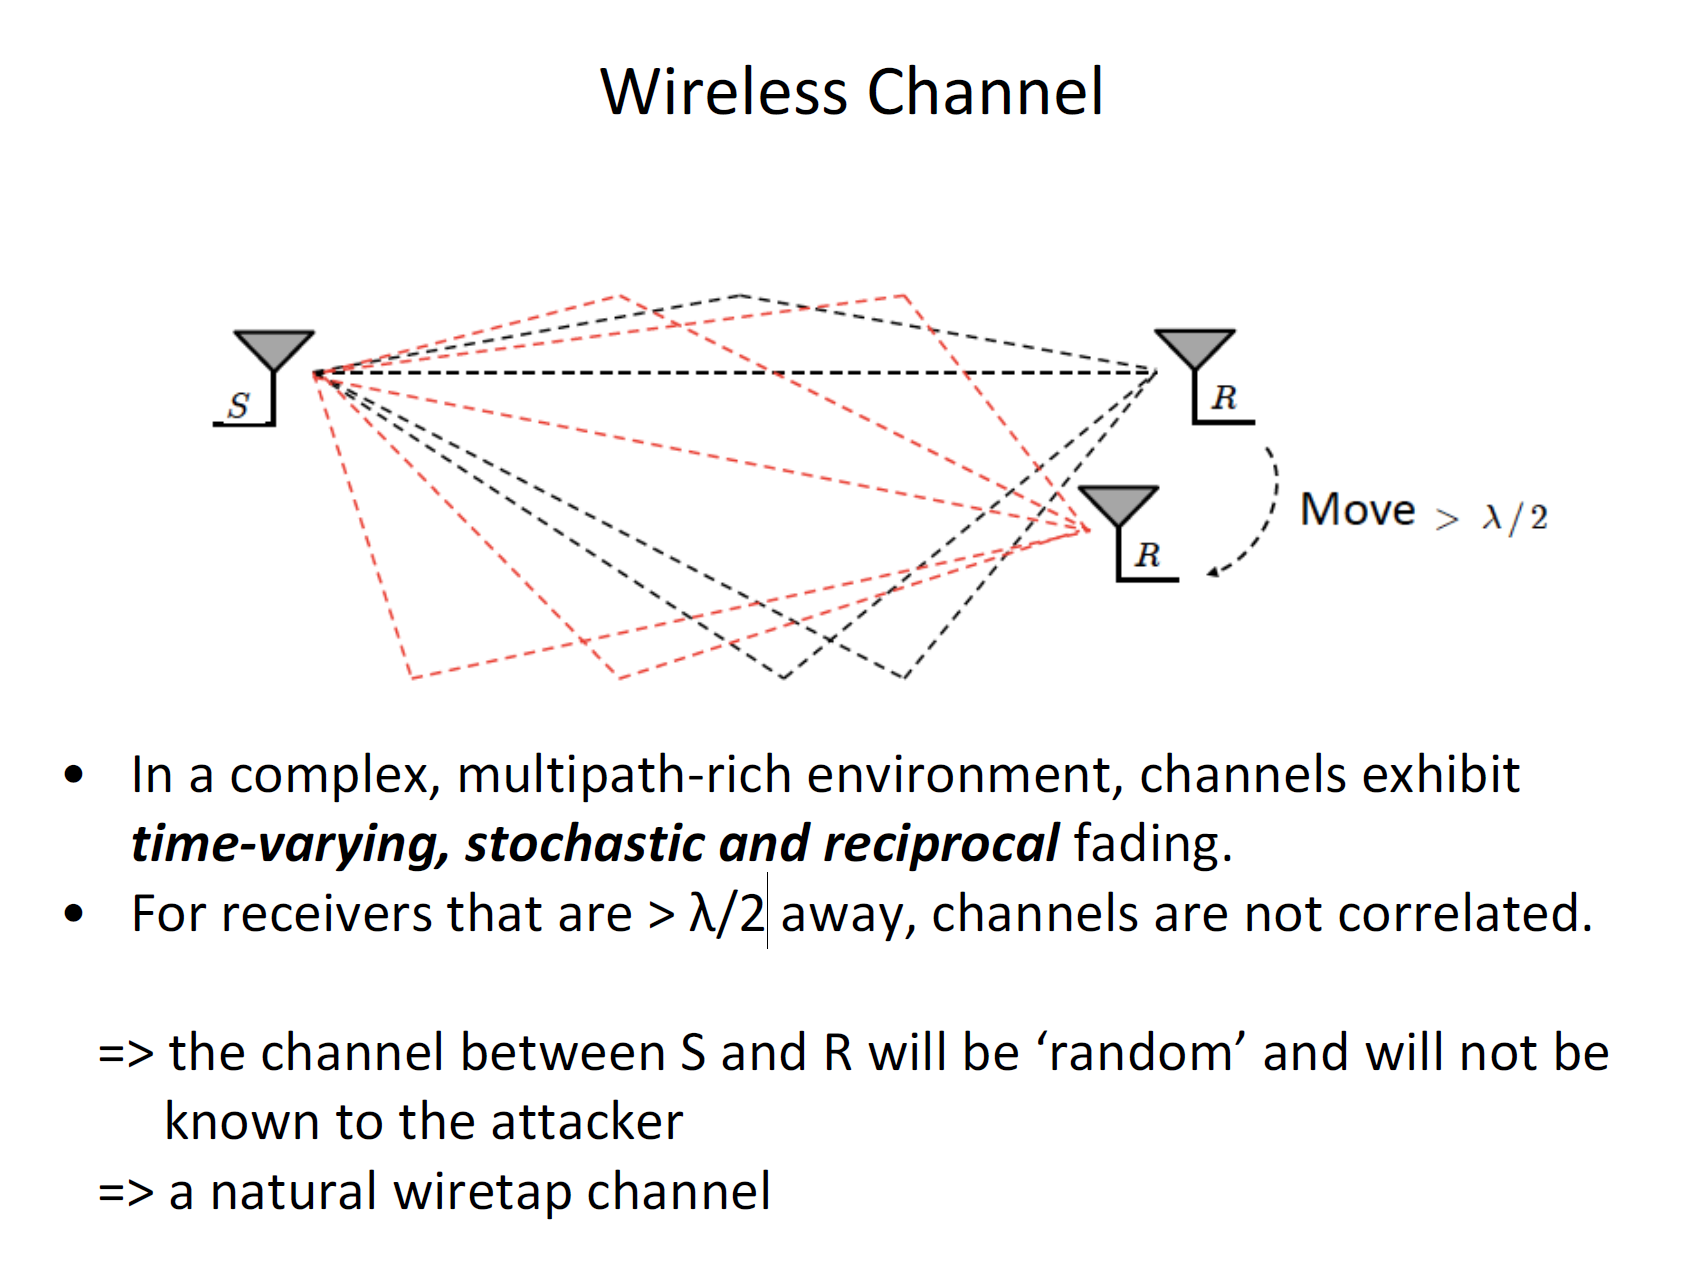
\includegraphics[width=\linewidth]{Figures/L7_channel.PNG}
\end{minipage}

The attacker does not know and cannot remotely measure multipath fading components, however both communication participants have the same fading. Use this for key agreement protocol. Fading is measured using Channel impulse response (CIR).

\begin{enumerate}
    \item S sends a well-known signal to R
    \item R detects the difference from received signal to expected signal, which correspond to the fading.
    \item R sends the same signal to S, and he computes the fading. Now both have a random symmetric random fading component, which they can use to derive a key.
\end{enumerate}

\begin{minipage}{\linewidth}
    \centering      
    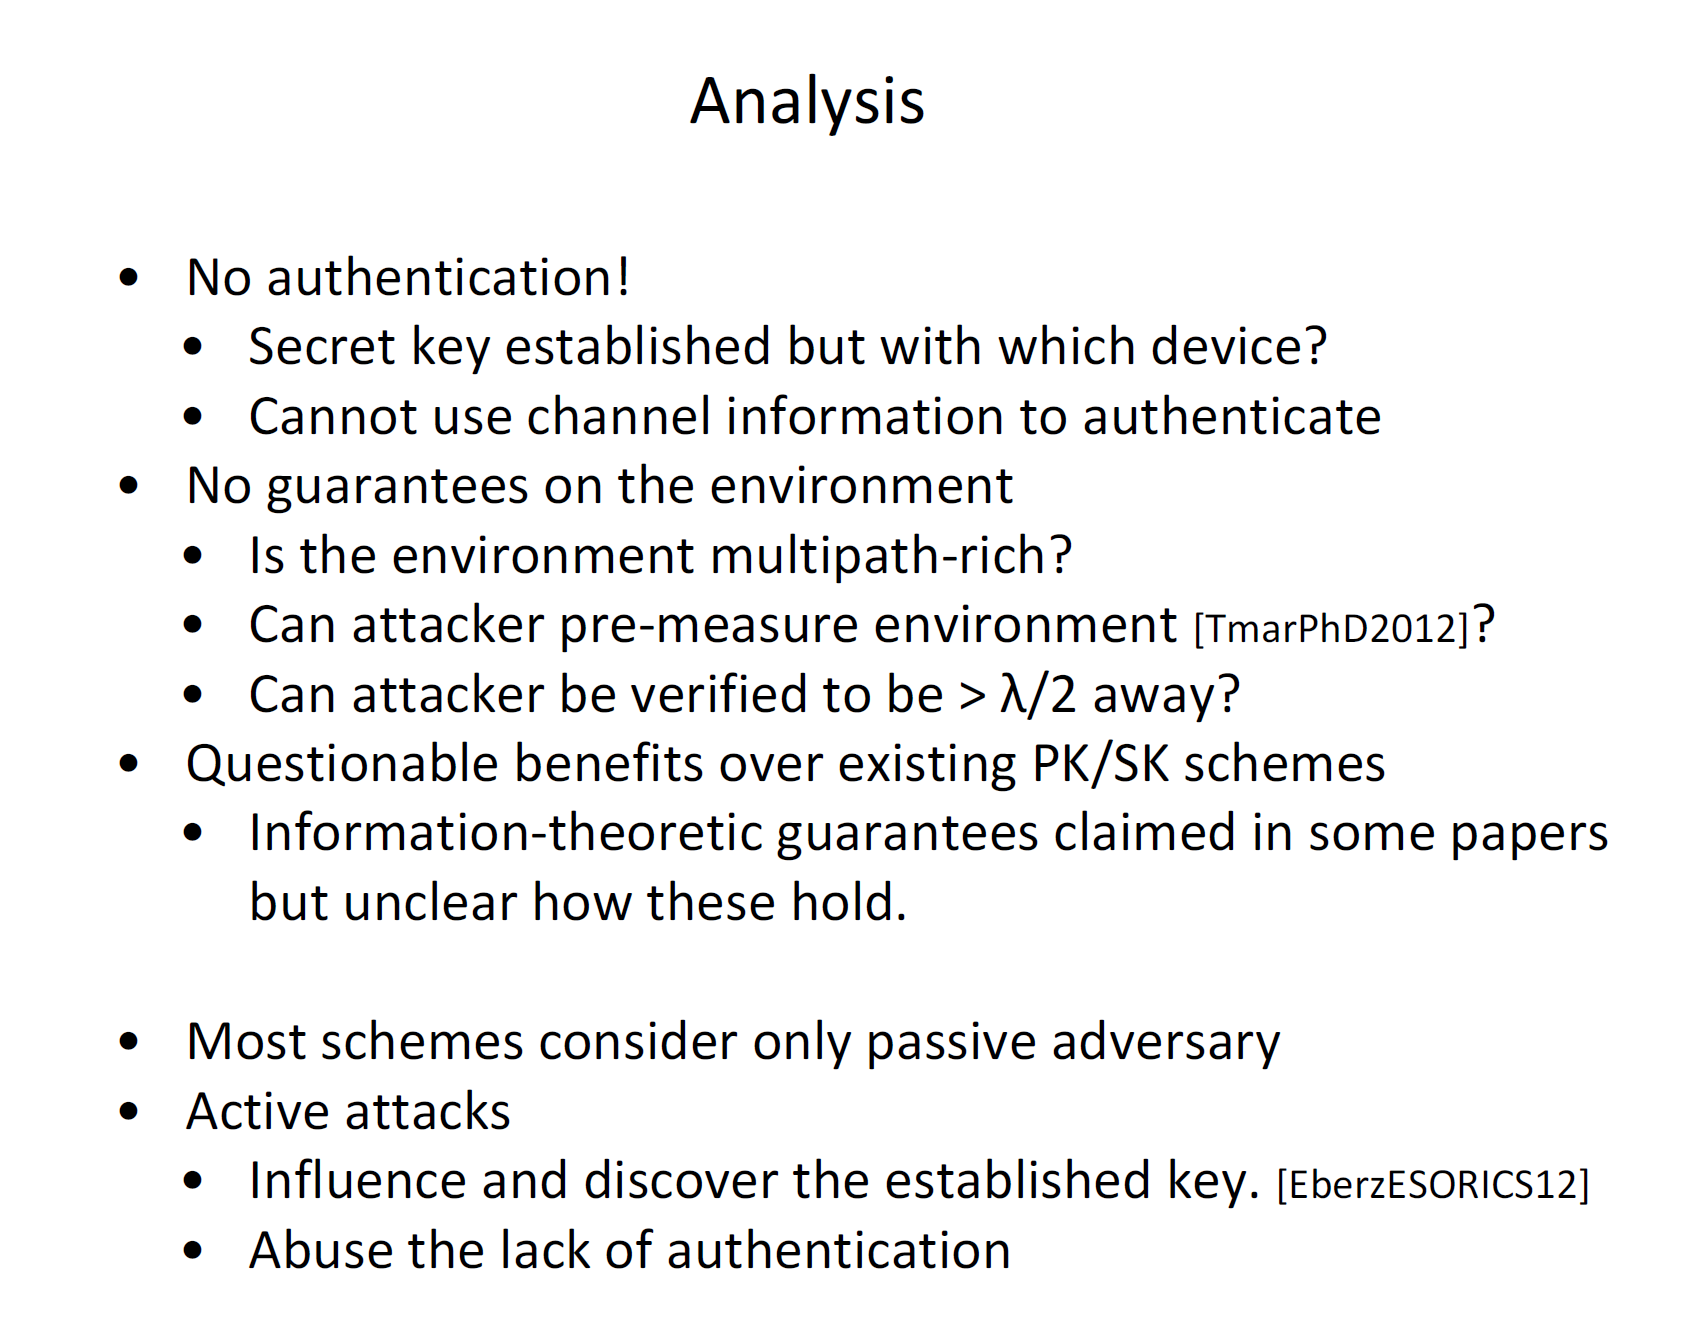
\includegraphics[width=\linewidth]{Figures/L7_channel_analysis.PNG} 
\end{minipage}

\subsection{Ensuring Secrecy with Multiple Input Multiple Output Antennas (MIMO)}
By using multiple antennas the sender can:
\begin{itemize}
    \item steer the signal towards the receiver and away from the attacker.
    \item Use jamming to interfere with the attacker, but not with the receiver.
\end{itemize}

\paragraph{Modeling the Channel}
\begin{itemize}
    \item At the receiver, signal has different phase and amplitude
    \item Channel is modeled as a single complex number:
    \begin{itemize}
        \item Captures both change in amplitude (real part) and phase (imaginary part).
        \item Represents cumulative effects of all multipath components.
    \end{itemize}
\end{itemize}

\subsubsection{Zero Forcing}
\begin{minipage}{\linewidth}
    \centering      
    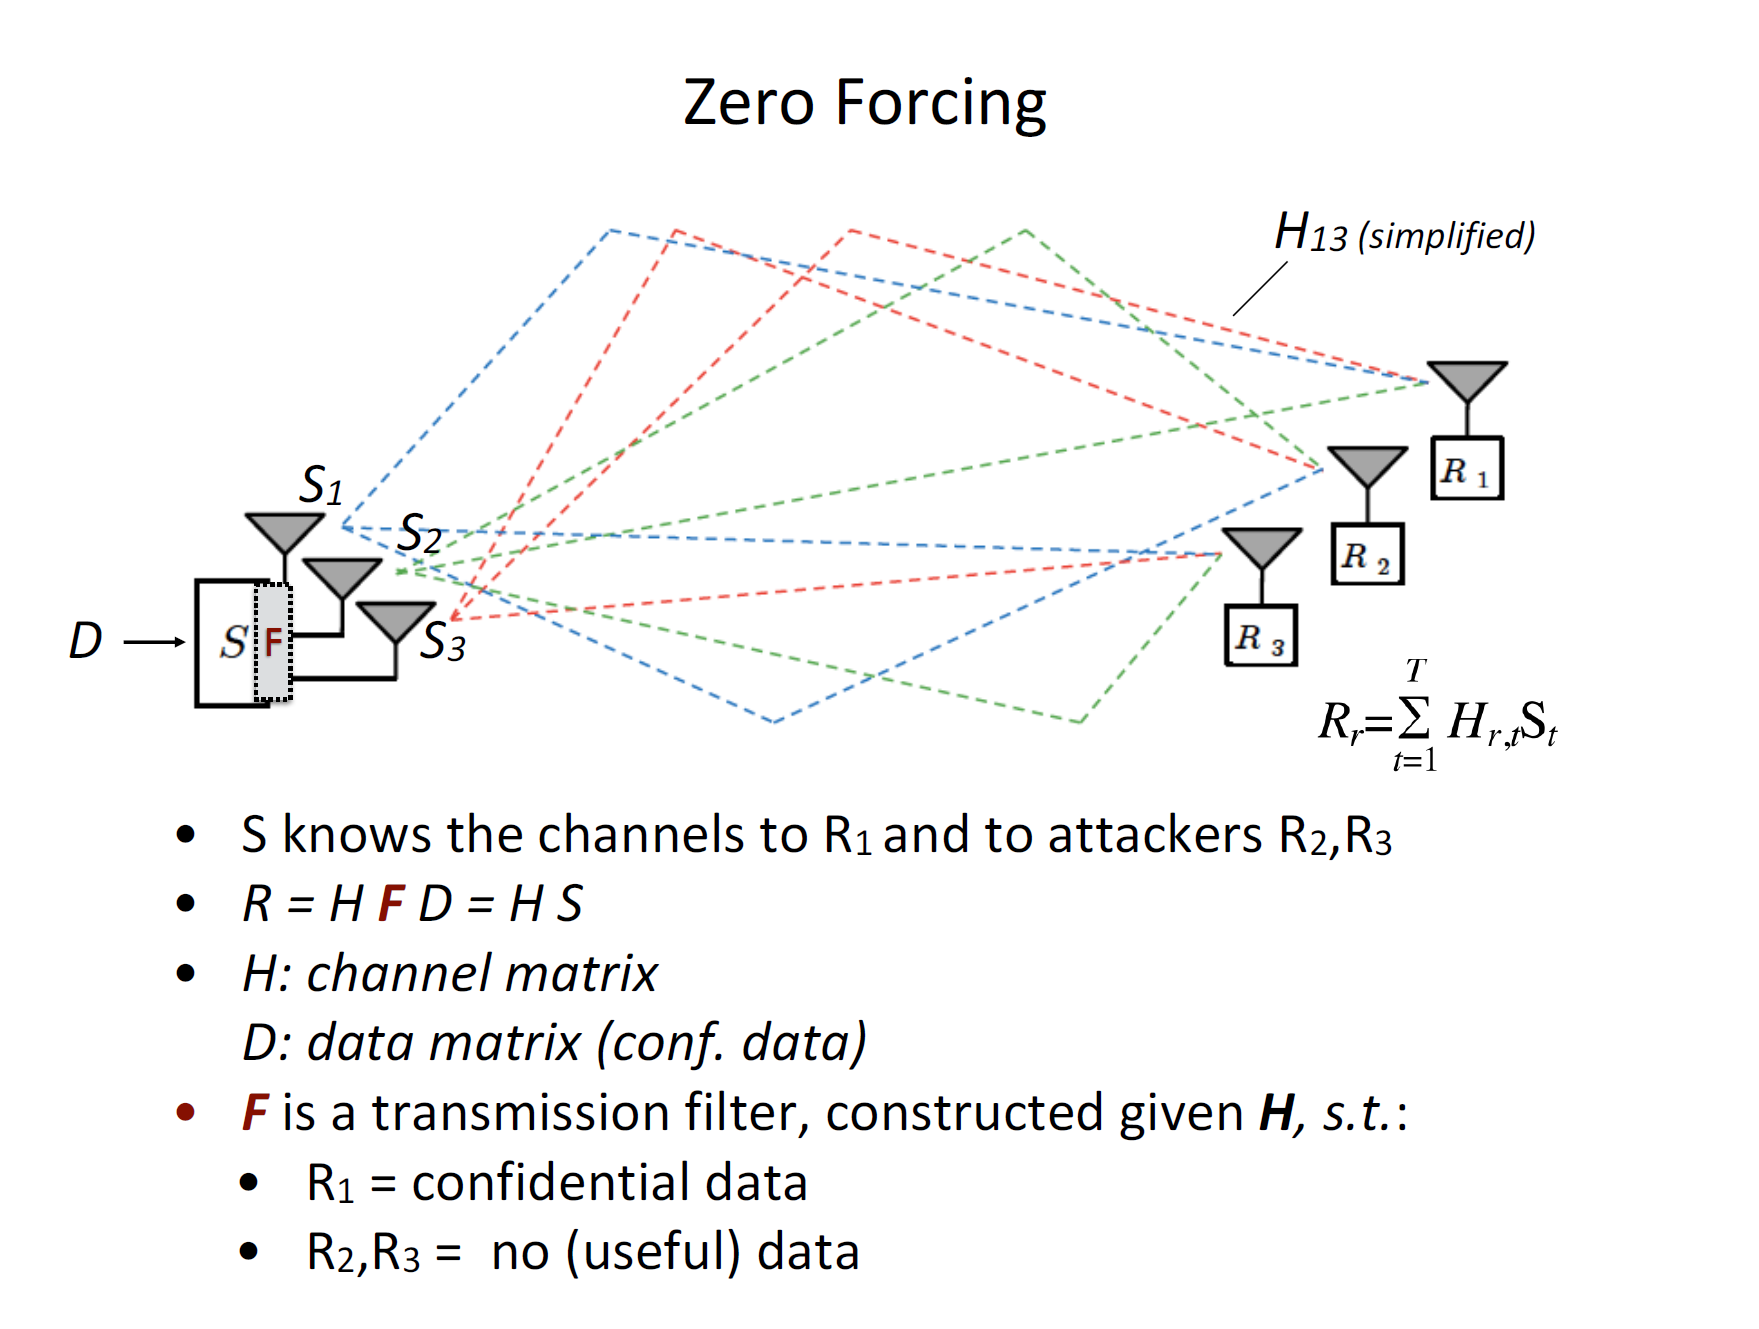
\includegraphics[width=\linewidth]{Figures/L7_zero_forcing.PNG} 
\end{minipage}

\subsubsection{Orthogonal Blinding}
In this scenario the sender knows the channel to the legitimate receiver, but does not know the channels to the attackers around (more realistic scenario). Thus he only knows partial entries of H (H would contain the channels to all possible receivers not only the legitimate one). The sender will randomly generate the missing parts of H in such a way that most surrounding attackers would be jammed and R receives confidential data.
\begin{minipage}{\linewidth}
    \centering      
    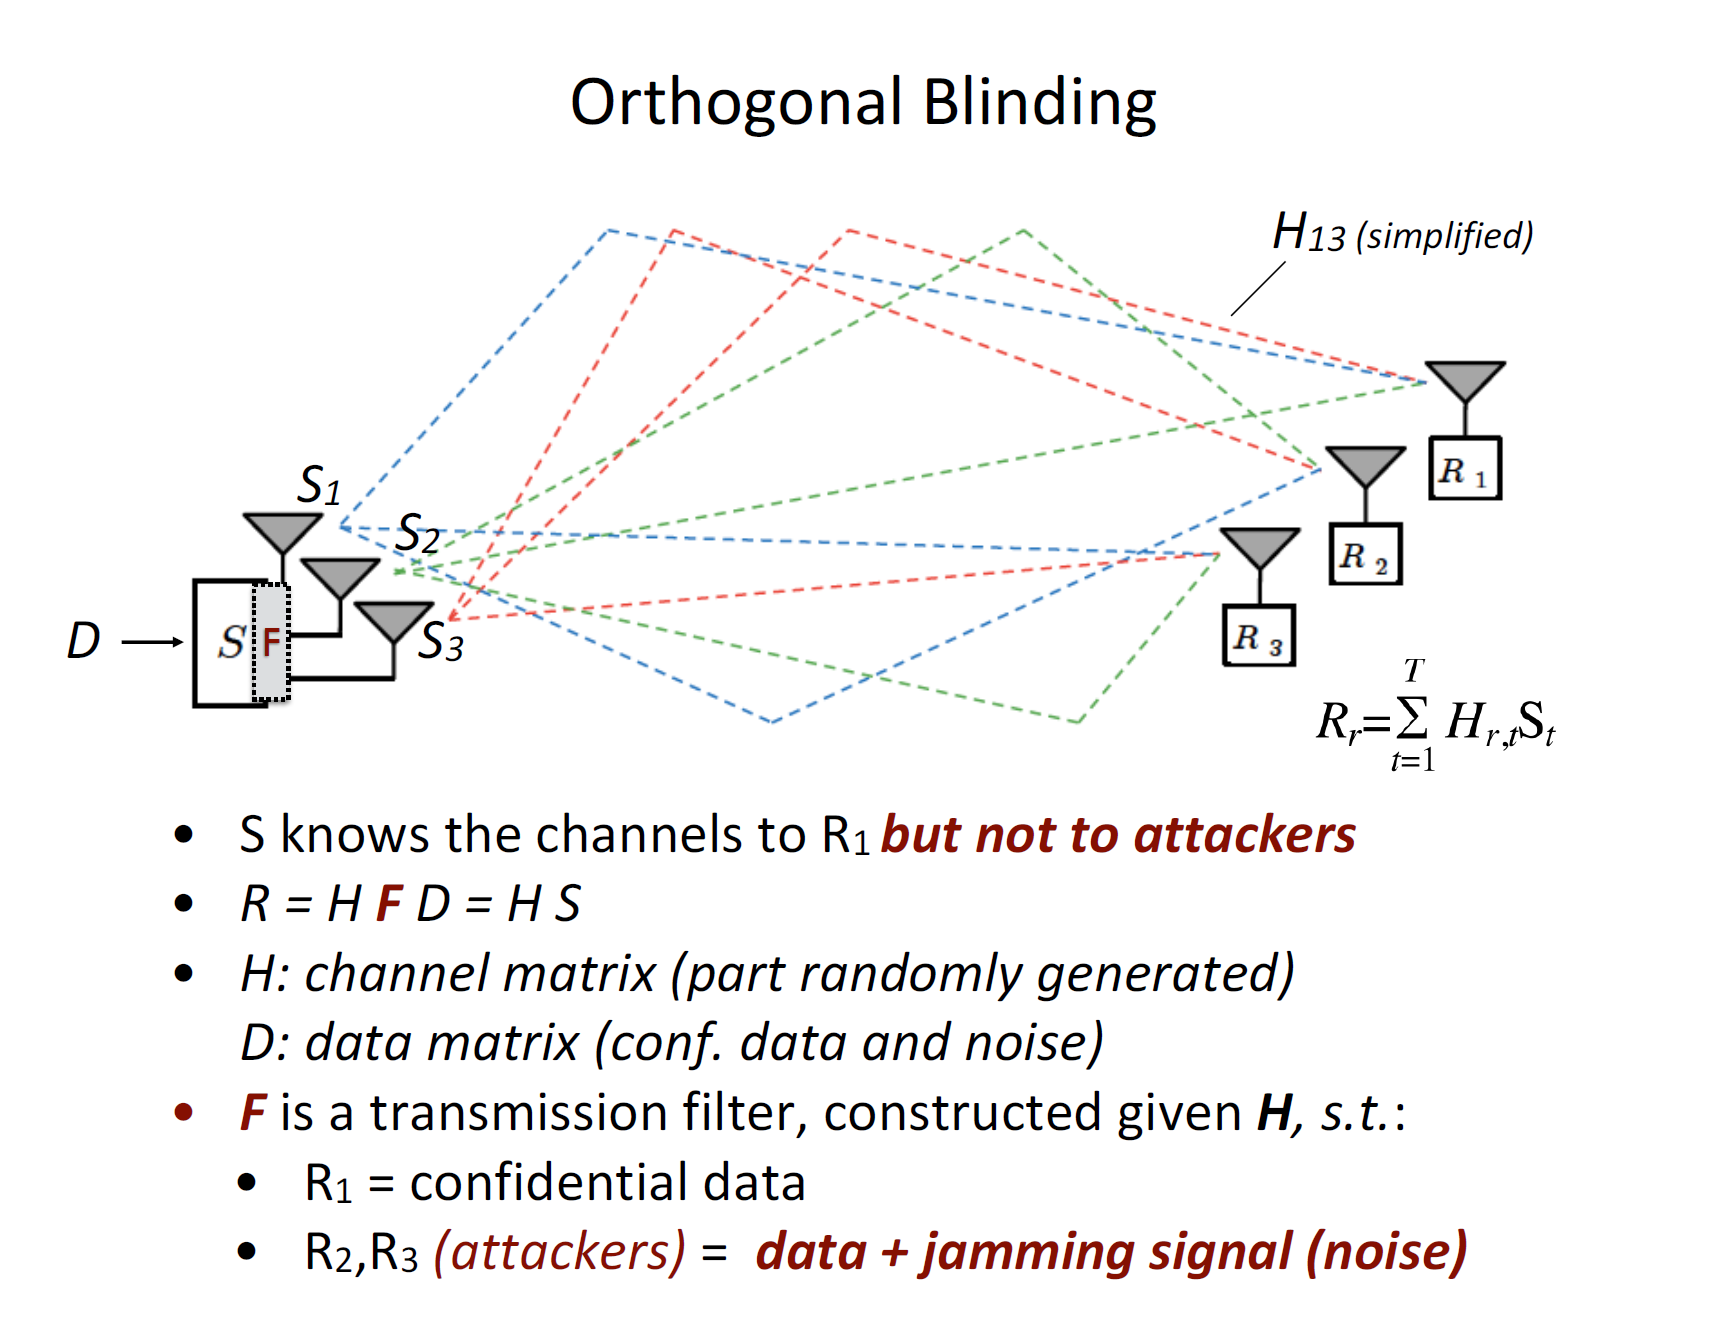
\includegraphics[width=\linewidth]{Figures/L7_orthogonal_blinding.PNG} 
\end{minipage}

\begin{minipage}{\linewidth}
    \centering      
    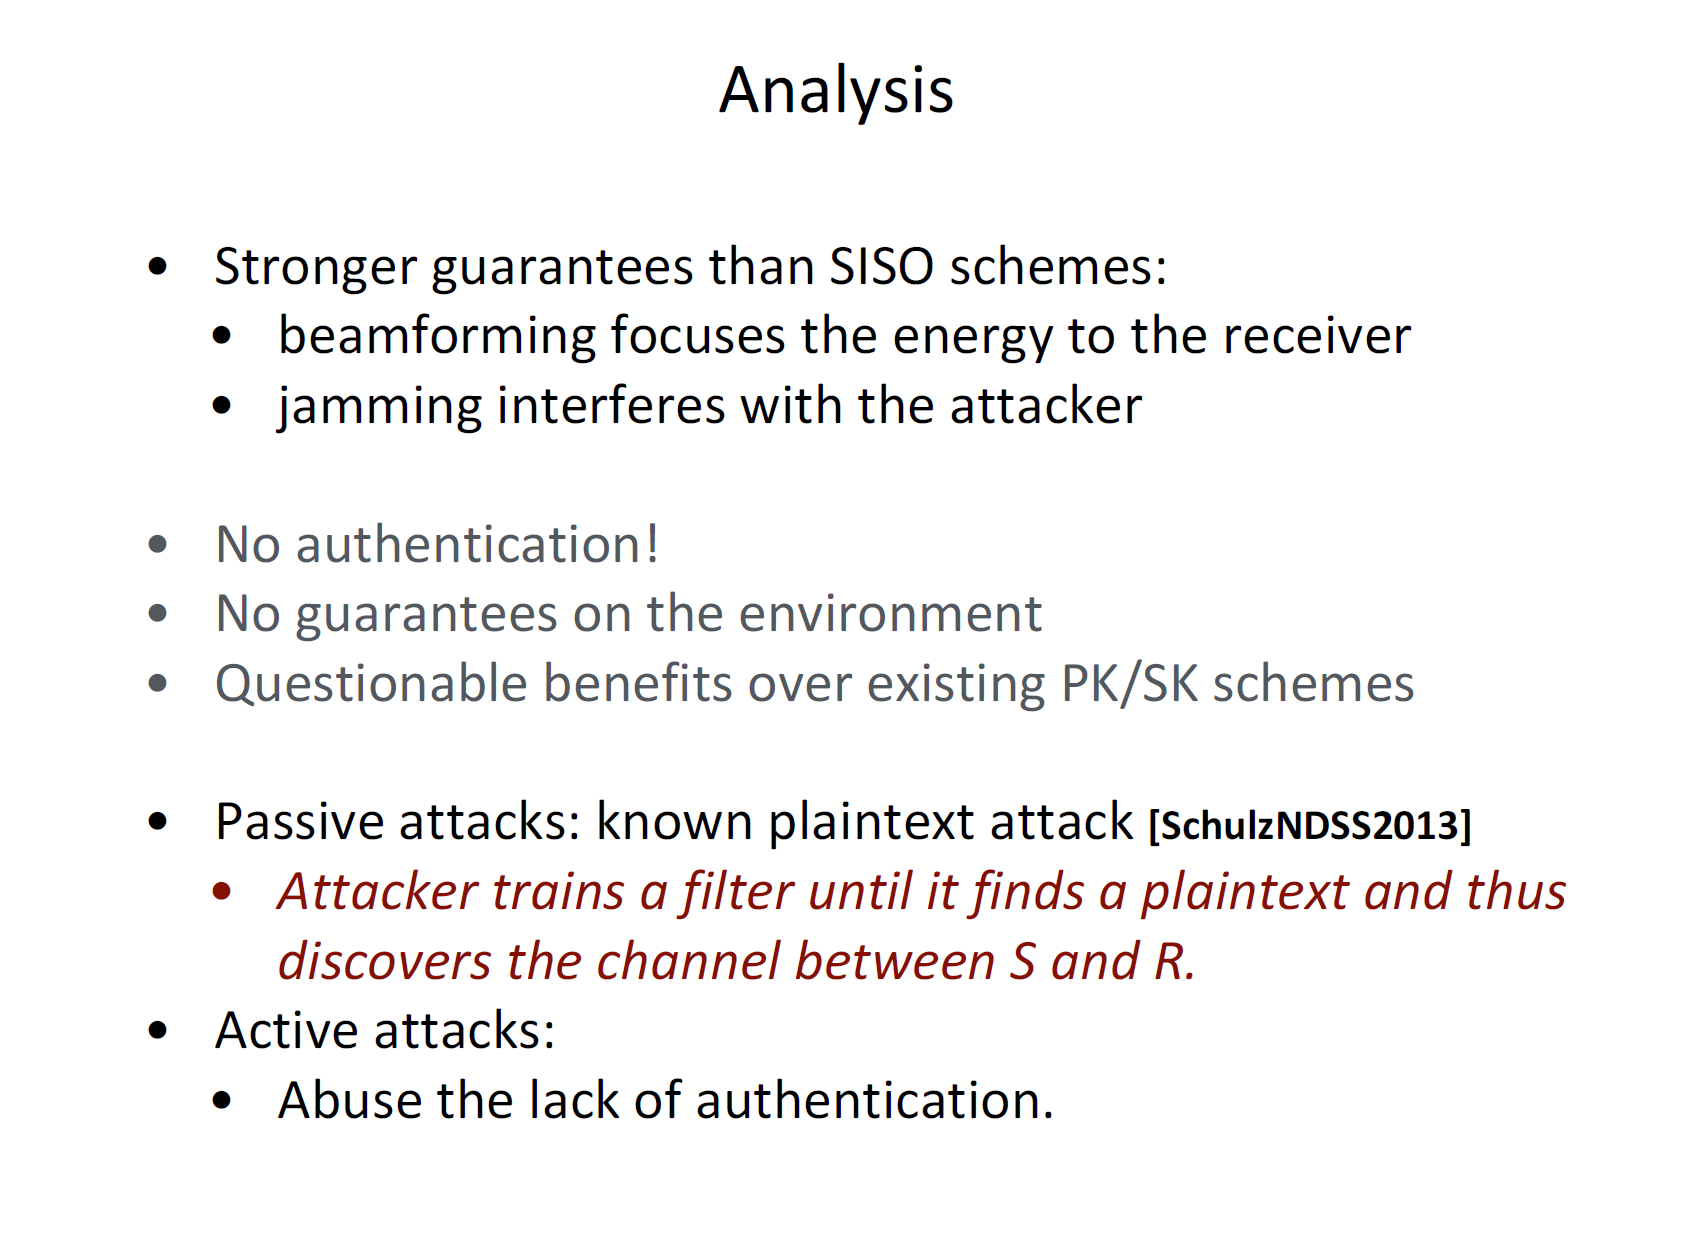
\includegraphics[width=\linewidth]{Figures/L7_secrecy_analysis.PNG} 
\end{minipage}
SISO = single input single output (single antenna)

\subsection{Jamming for Confidentiality}

\paragraph{Orthogonal blinding / Zero forcing:}
Transmit noise into the null-space of the receiver's channel.
\begin{itemize}
    \item no pre-established secrets
    \item used for key establishment
\end{itemize}

\paragraph{Friendly Jamming:}
Transmit noise which the receiver subtracts
\begin{itemize}
    \item Receiver know the seed used tog enerate the noise.
    \item Eavesdropper cannot seperate signal and noise.
    \item Jamming signal is much stronger and covers the spectrum of the data signal.
    \item If distance between jamming antenna and signal antenna (both at sender) $> \lambda/2$, attacker equipped with two antennas can seperate signals from J and D (different channels)
    \item I distance beween tscheggi nöd sl. 18
\end{itemize}

\paragraph{Example IMD Shield}
IMD shield jams the eavesdropper, but also legitimate readers, however shield can be removed.

\paragraph{Friendly Jamming Security Arguments:} 
Security properties in the friendly jamming scenario.

\begin{minipage}{\linewidth}
    \centering      
    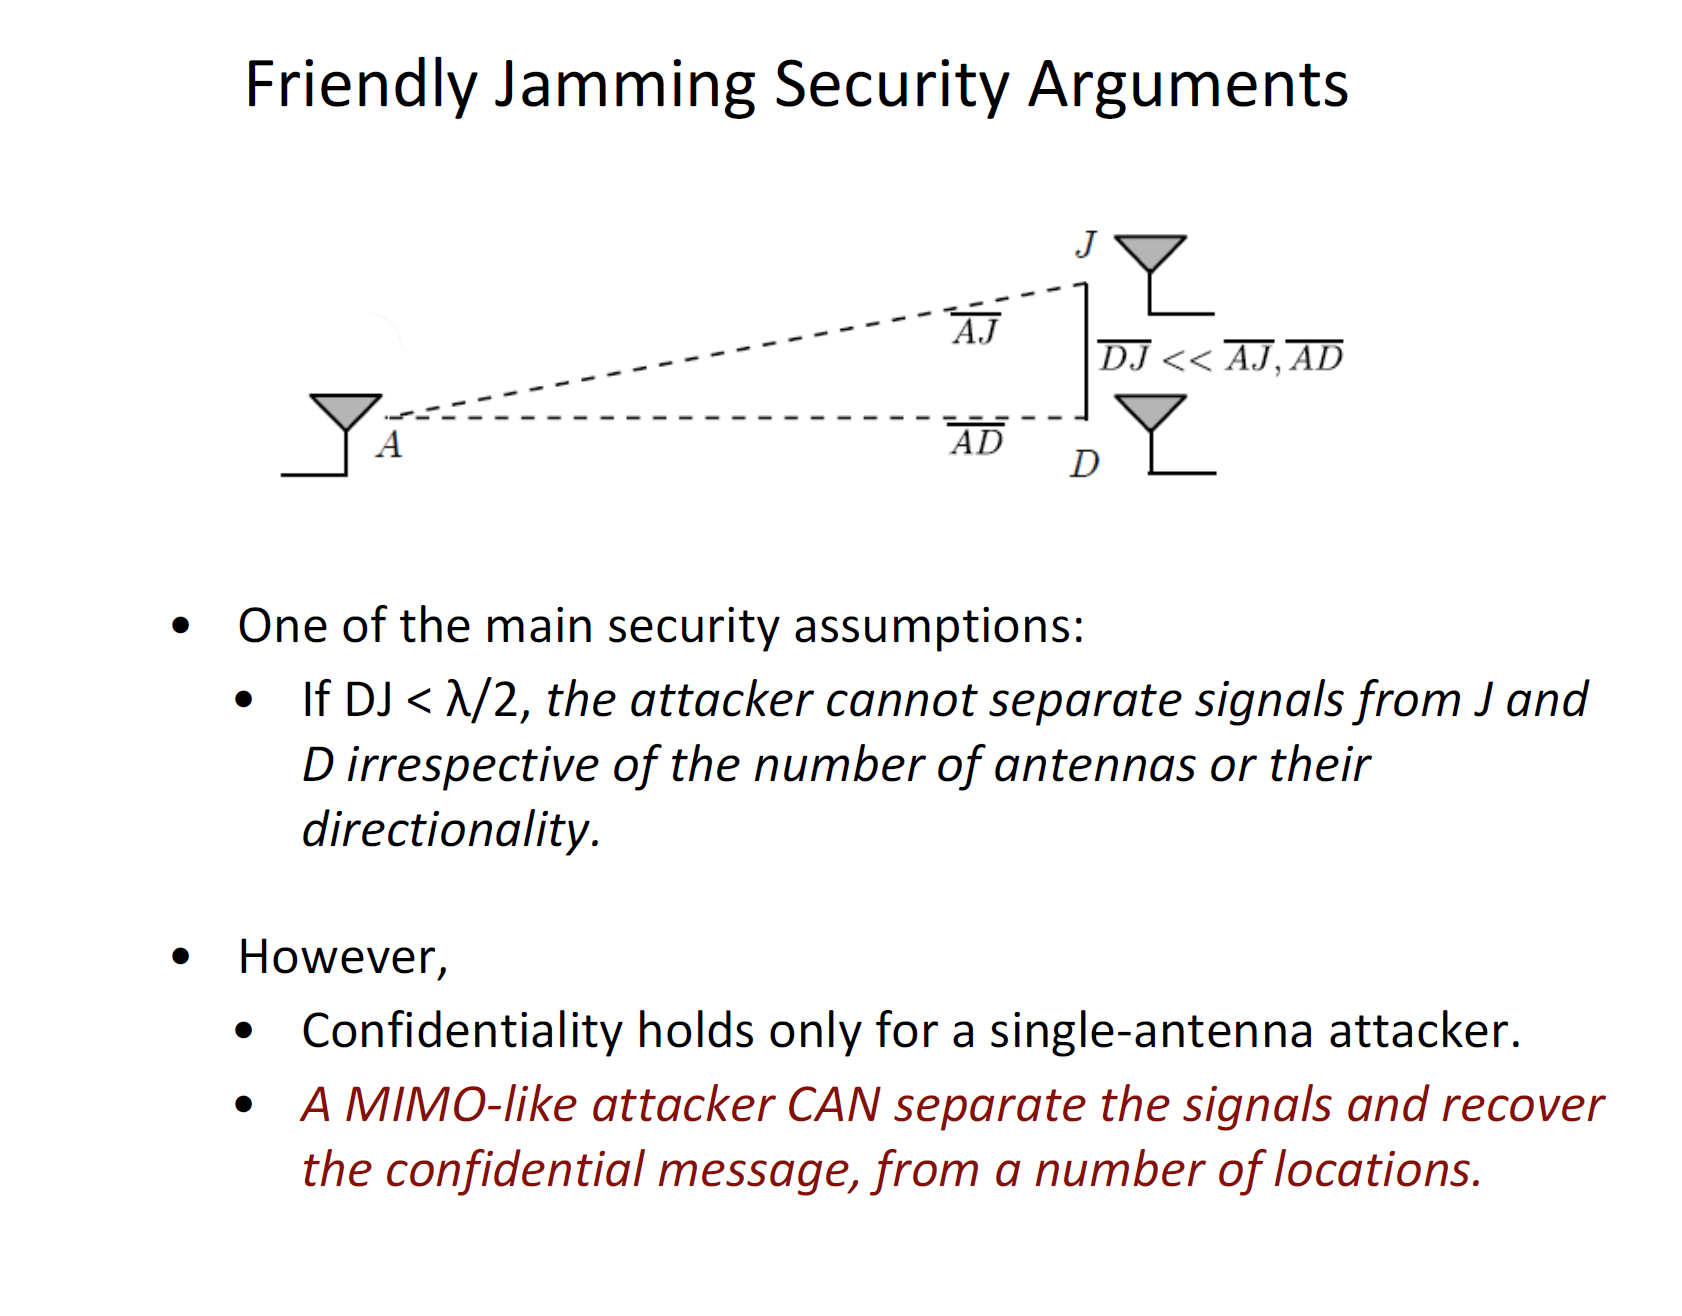
\includegraphics[width=\linewidth]{Figures/L7_friendly_jamming_security.PNG} 
\end{minipage}

Note: A MIMO-like attacker can seperate the jamming and data signal as long as they do not stem from the same antenna, as is the case in the IMD Shield. This is the case because the two signals J and D have different arrival times at the two antennas of the attacker, which makes them distinguishable at ideal attacker placements.

\paragraph{Multipath:} So far, we looked at line of sight (LOS) channels, no reflections (at least for friendly jamming) 
\begin{itemize}
    \item Multipath will introduce more variation of amplitudes of components.
    \item Change the phase offsets of the signals.
    \item Potentially prevent us from cancelling the jamming signals, so we have stronger guarantees.
\end{itemize}

\paragraph{Lessons Learned}
Using Jamming for confidentiality is not without risk.
\begin{itemize}
    \item MIMO-like attacker can retrieve data despite DJ < $\lambda/2$
    \item The attack work from many locations (with some post-processing)
    \item The attack can be effective even when jammer and source are mobile.
    \item Note: Friendly jamming works well for access control in the sense that it is very hard for the attacker to make its signal receive the device under consideration.
\end{itemize}

\paragraph{Signal Manipulation}
Simple setup with two directional antennas, one directed to the sender and one to the receiver, creates artificial multi path that suppresses the transmitted signal at the receiver. The receiver does not know that any message was even sent by the transmitter.

\subsection{Broadcast Authentication}
Integrity Codes: Broadcast Authentication base on Presence Awareness.

\paragraph{Setup:} Broadcaster (known to be present and sending at known channel frequency) and listeners that do not have pre-shared keys or distributed credentials (e.g. certificates/ public keys). Example would be an AP in the airport broadcasting its public key in presence of a potential rogue AP, that tries to send rogue public keys.

\begin{minipage}{\linewidth}
    \centering      
    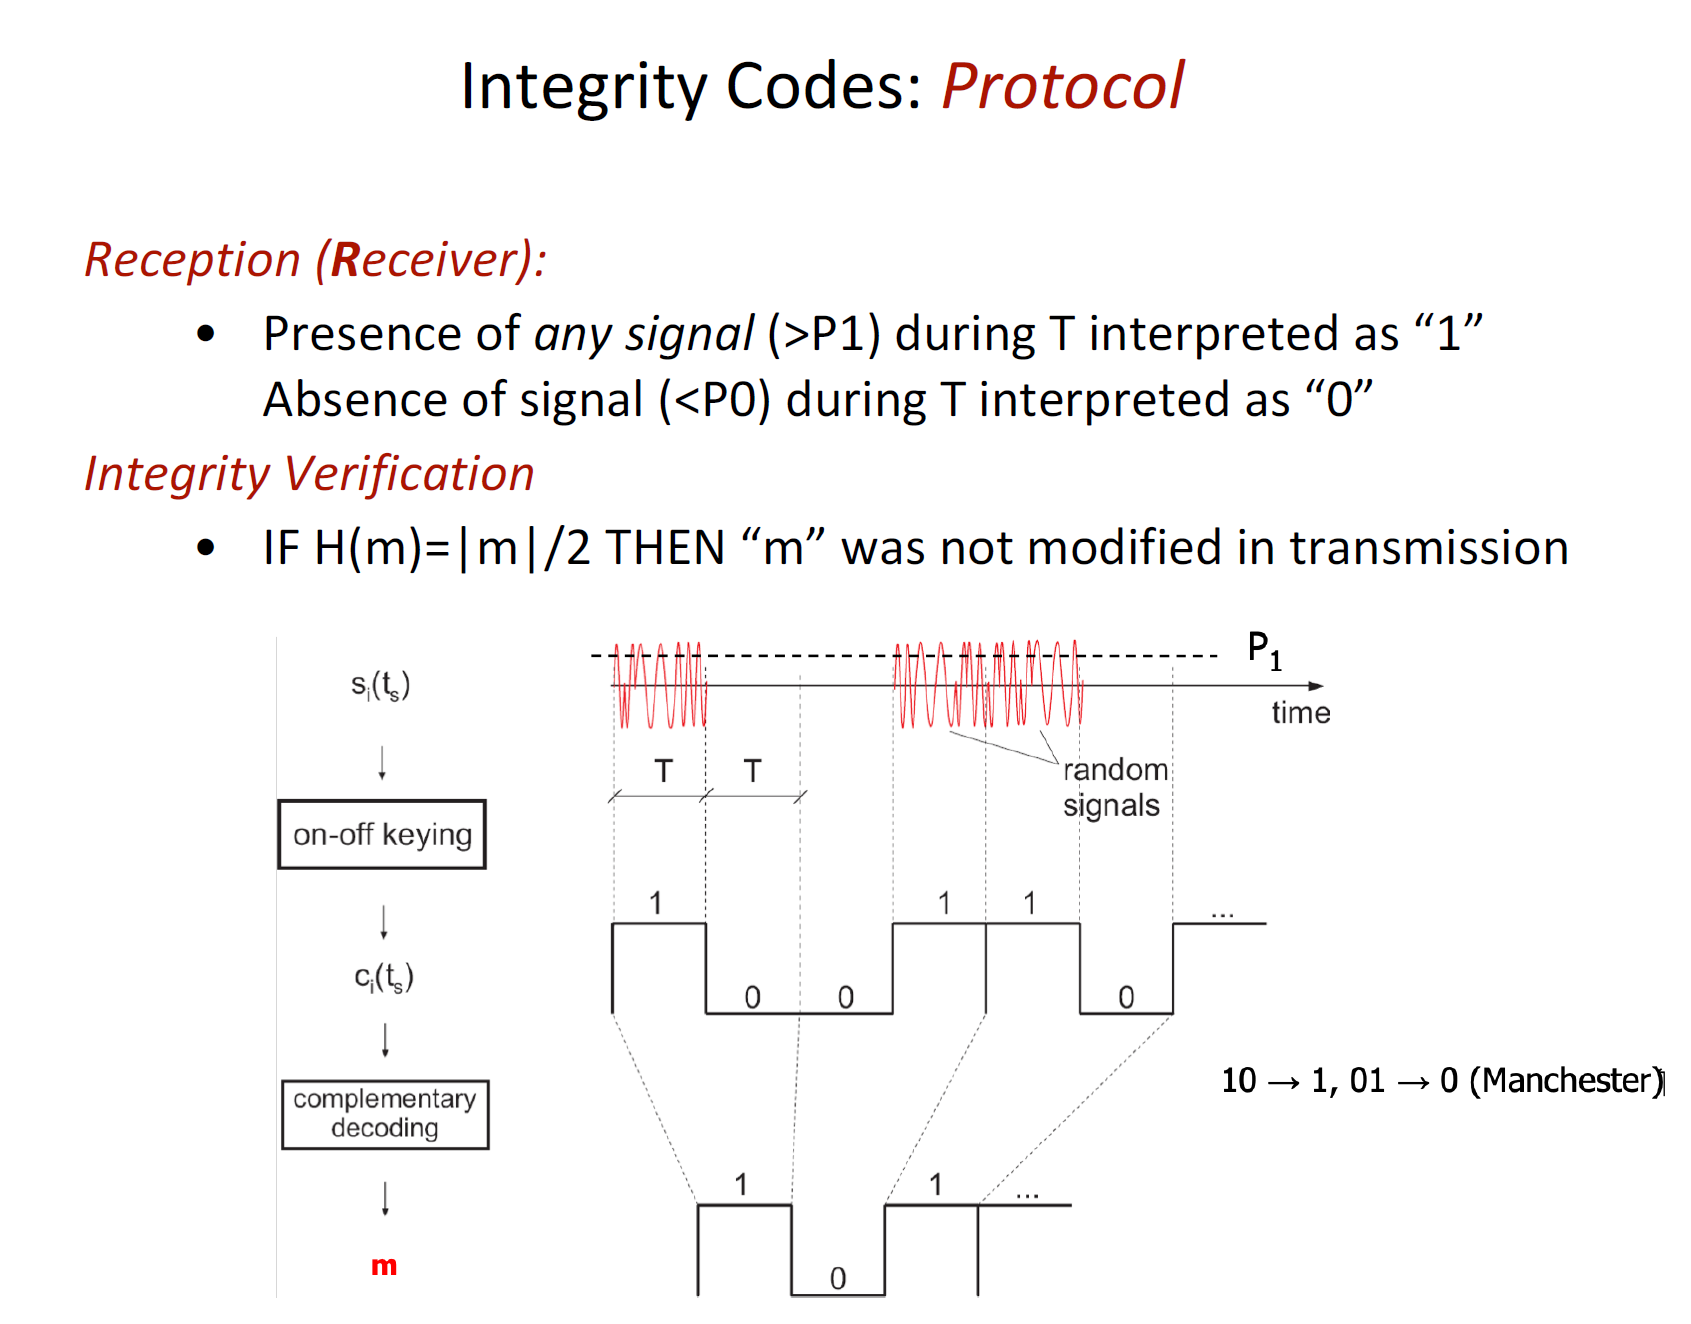
\includegraphics[width=\linewidth]{Figures/L7_integrity_codes.PNG} 
\end{minipage}

Now attacker can only inject 1, assuming he cannot cancel out the amplitude of existing 1s. However injected 1s result in non equal numbers of 1s and 0s, so it can be detected.
